\begin{figure}[t]
  \centering
 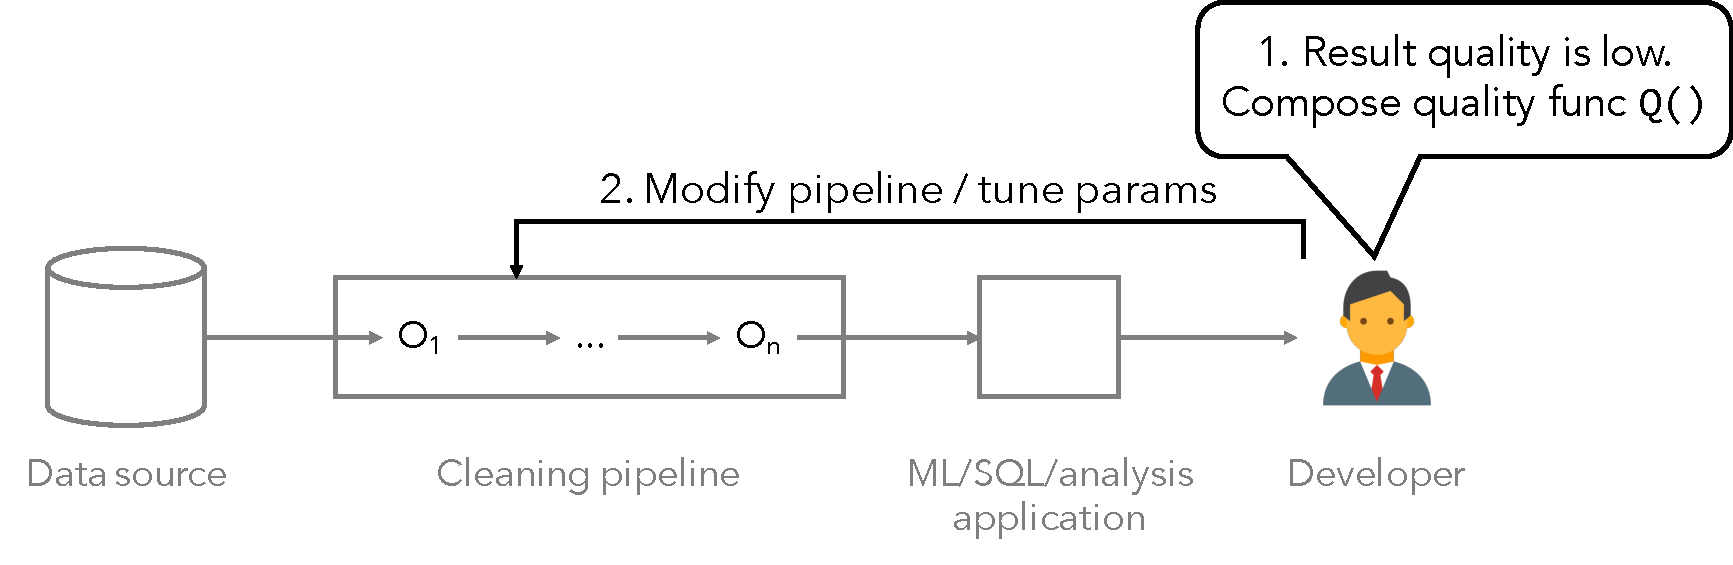
\includegraphics[width=\columnwidth]{figures/user-pipeline}
 \caption{\small Typical data cleaning pipeline.  The user finds that analysis results (of SQL query, ML model, web application, etc) are suspicious and iteratively (1) composes a quality function to characterize the suspicious quality issues, and (2) modifies the data cleaning pipeline to address the errors.  \sys improves this human-in-the-loop process by providing an expressive, composable quality function, and automatically searching for cleaning pipelines.  \label{fig:user-pipeline}}
\end{figure}


\section{Background}\label{s:background}
We will use the example illustrated in Table \ref{example} to convey the concepts in \sys.  The \red{red} cells indicate value errors that need to be fixed.

\begin{example}[Detecting Errors]\it\label{e:1}
Lisa finds that her application that uses the \texttt{City} table produces strange results. From a cursory examination of table, she finds that the city name and code are not always consistent with each other.  Thus, she tests the functional dependency \texttt{city\_name$\rightarrow$city\_code}. Unfortunately, the functional dependency test does not capture all of the data errors. When she examines the distribution of city names, she finds also finds large number of singleton city names, such as \texttt{San Francisco:SF}, which satisfy trivial functional dependencies. She realizes that \texttt{ispell} program can be used to detect further errors through spell checking the \texttt{city\_name} attribute.
\end{example}

  \begin{table}[t]
	\small
  \centering
  \begin{tabular}{|l|l|l|}
  \hline
  \rowcolor[HTML]{000000} 
  & \white{name}            & \white{code}   \\ \hline
  1 & \red{\textbf{San Francisco:SFO}}                    &    \red{\textbf{`'}}                               \\ \hline
  2& \red{\textbf{New York}}           & NY                                  \\ \hline
  3 & New York City                    & \red{\textbf{NYC}} \\ \hline
  4 & \red{\textbf{San Francisc}}      & SF                                  \\ \hline
  5 & San Francisco                         & SF                                 \\ \hline
  7 & New York City                    & NY                                  \\ \hline
  \end{tabular}
    \caption{The \texttt{City} relation contains two attributes \textsf{name} and \textsf{code}. 
Some of the cells contain errors highlighted in \red{red}. \label{example}}
  \end{table}

\subsection{Data Cleaning Libraries}
Example \ref{e:1} highlights a few key points. First, data cleaning is iterative. The developer explores a large space of possible data quality issues {\it and} and iterates until she covers all of the apparent anomalies in a dataset (Figure \ref{fig:user-pipeline}). Second, data quality is not solely determined by integrity constraint satisfaction. In the example above, the user actually uses the number of singleton city names and spelling errors as a \emph{proxies} for data quality. The combination of these metrics with the functional dependency violations allows her to effectively detect errors.

The data cleaning software ecosystem is diffuse, with separate frameworks for constraint resolution ~\cite{rekatsinas2017holoclean}, cleaning in machine learning pipelines~\cite{DBLP:journals/pvldb/KrishnanWWFG16}, entity resolution~\cite{mudgal2018deep, doan2018toward}, and crowdsourcing~\cite{DBLP:journals/pvldb/HaasKWF015}.
Therefore, the iterative data cleaning process is not just tuning a single framework but also understanding how the different frameworks interact.
Each of these frameworks has its own idiosyncrasies and parameters, and tuning even one of them can be a daunting challenge.
Real-world datasets have mixes of errors~\cite{krishnan2016hilda} and often require multiple different libraries to clean~\cite{DBLP:conf/sigmod/ChuIKW16}.

Although the availability of open-source data cleaning software makes it easier to construct and execute a pipeline, the space of possible compositions, the parameters, and pipeline depth is infeasible for developers to manually search.
While a single, unified automated data cleaning system may not be possible, a reasonable compromise is a tool that allows analysts to efficiently compose different libraries together.
This paper proposes such a tool where the quality of each possible composition will be assessed by weighted combinations of user-specified quality metrics (e.g., FD violations, spelling errors, and distributional anomalies).


\begin{figure}[t]
\centering
 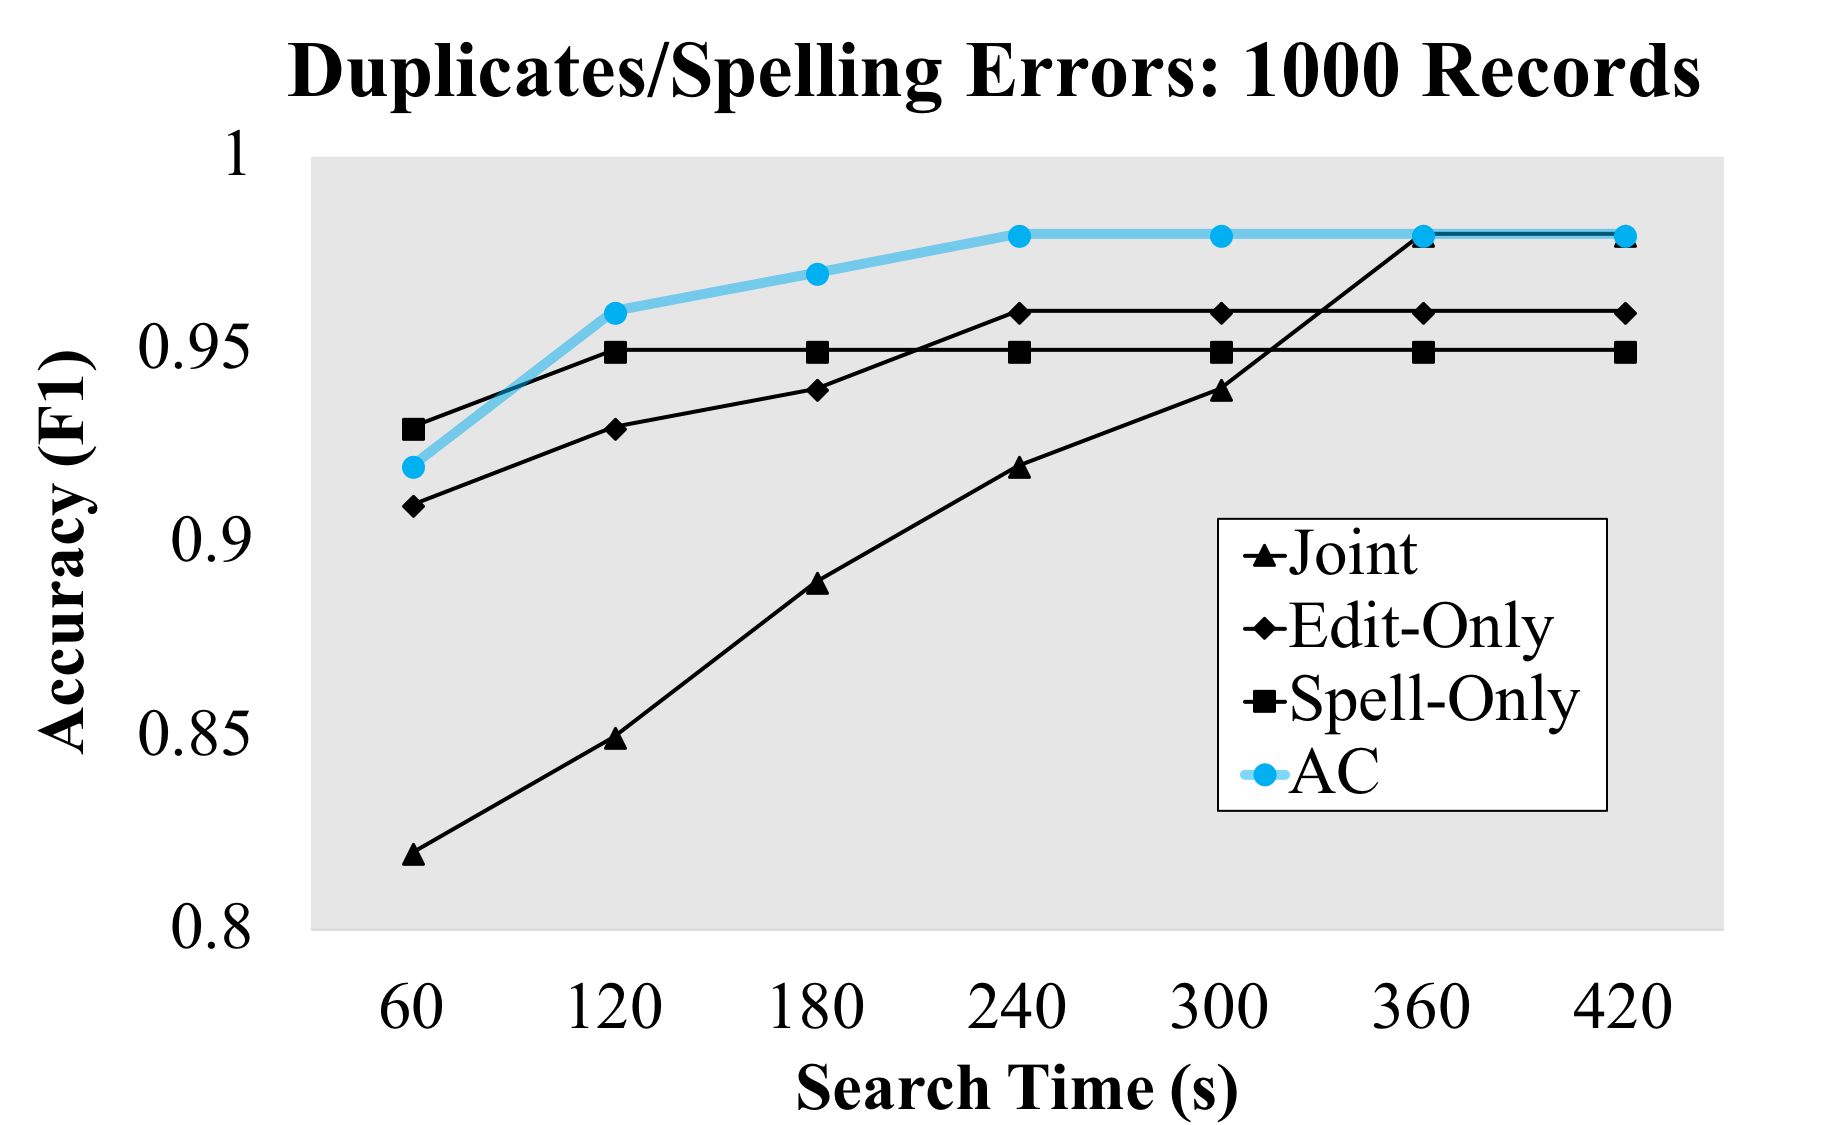
\includegraphics[width=0.9\columnwidth]{figures/teaser-experiment.png}
 \caption{\small 10\% of a dataset of dictionary words are duplicated with randomly generated spelling errors. The dataset is to be cleaned with a similarity matcher and a spell checker. Holistically, tuning the parameters of both with \textsf{python hyperopt} (BB-Full) is inefficient due to interactions between the two data cleaning options. It takes over 3x the amount of search time for the joint optimization to exceed the best tuned single cleaning method (BB-Edit and BB-SpellCheck) \label{fig:teaser}}
\end{figure}

\subsection{Naive Hyperparameter Tuning}
We could start by considering the recent work in \emph{hyperparameter tuning} for machine learning, which identifies the optimal assignment of hyperparameters to maximize an objective function (e.g., training accuracy for ML models).
Several systems have been built to run hyperpameter and neural network model search at scale~\cite{li2017hyperband, sparks2017keystoneml, baylor2017tfx, golovin2017google, liaw2018tune}.
For single threaded search, the state-of-the-art remains to be Bayesian optimization, e.g., Python Hyperopt~\cite{bergstra2013hyperopt}.
Since Bayesian optimization is inherently sequential, for parallel and distributed settings, the community is increasingly studying randomized and grid search schemes~\cite{li2017hyperband, liaw2018tune, golovin2017google}.
 
The main issue is what we call ``the attribution problem'', namely, which parameter change is responsible for an increase (or decrease) in objective value.
Figure~\ref{fig:teaser} illustrates this concern on a toy data cleaning problem, with a hyperparameter search based on Tree-structured Parzen Estimator (TPE)~\cite{shahriari2016taking}\footnote{Implemented using \textsf{python hyperopt}}.  We corrupted 1000 dictionary words so that 10\% are duplicated with randomly generated spelling errors affecting 1-3 characters. The quality function is the F1 score of the cleaned dataset as compared to the ground truth.  We consider two parameterized operators: \texttt{edit\_dist\_match(thresh)} is a string edit distance similarity matcher with a tunable threshold, and \texttt{ispell(rec)} is a spell checker with a tunable recommendation parameter based on the distance between the dictionary word and the misspelled word.  The two operators partially overlap in their cleaning behavior, and we will see how it affects the search problem below.   

We compare hyperparameter search for three fixed pipelines:  single-operator pipelines (\texttt{edit\_dist\_match}) and (\texttt{ispell}), and a joint pipeline (\texttt{edit\_dist\_match}, \texttt{ispell}).  By fixing the operator pipeline, the search algorithm only needs to learn parameterizations of the operators.  Although we expect the joint pipeline to perform the best, Figure \ref{fig:teaser} shows that there is a trade-off between runtime and data quality (measured as F1 score).  It takes 3$\times$ amount of search time for the joint pipeline to exceed the best single-operator pipeline.    In contrast, the single operator pipelines quickly converge to an F1 score of $\ge95\%$.  The reason is because the two operators overlap in functionality (some duplicates can be fixed by \texttt{ispell} or \texttt{edit\_dist\_match}), which forces the join optimization to explore redundant parameter settings that have the same cleaning results.  In practice, pipelines and the set of operators can be much larger, thus the likelihood of redundant operators, or even operators that reverse changes made by previous operators, is high.

For example, what if we independently optimized both single-operator pipelines (\texttt{edit\_dist\_match}) and (\texttt{ispell}), and then took the consensus between their repairs?
Such operations are disallowed in current hyper-parameter tuning approaches. 
This is the main intuition behind \sys: rather than treating a pipeline as a monolithic parametrized unit, we decompose it into its constituent repairs.
The system then interleaves those repairs that improve the objective function.
These repairs can be generated asynchronously in a thread of workers that query each cleaning operator with different parameters--making it robust to operators that are slow or straggle on difficult datasets.
We also include the curve for when solving this problem with \sys on Figure \ref{fig:teaser}; the next sections describe the design to accelerate such cleaning problems.









